\section{Introduction to Language Modeling}
\large Language Modeling (LM) is about building systems that can understand, generate, or transform human language. At its simplest, a language model predicts the next word in a sequence based on the words that came before it. This ability forms the foundation of many applications in \textbf{natural language processing (NLP)}, such as chatbots (e.g., ChatGPT), machine translation, text summarization, and search engines. 

Let’s consider an example:

\begin{center}
    \textit{``The quick brown fox jumps \_\_\_.''}
\end{center}

Given this sentence, a language model would likely predict the word “over” as the next word, drawing on patterns it has learned from analyzing text. By recognizing and using patterns in language, these models can:
\begin{itemize}
    \item Complete sentences.
    \item Understand context.
    \item Generate coherent responses or paragraphs.
\end{itemize}

These are examples of text-generation tasks, where language models predict or create text based on input. Language models also support other types of NLP tasks, such as classification or summarization. 

Language models work by estimating the probability of a sequence of words. Formally, the model breaks this problem into smaller steps, predicting one word at a time based on the words before it:
\[
P(w_1, w_2, \dots, w_n) = P(w_1)P(w_2|w_1)P(w_3|w_1, w_2)\dots P(w_n|w_1, w_2, \dots, w_{n-1})
\]

This equation may look complex, but it simply means that the probability of an entire sequence is determined by multiplying the probabilities of each word, one after another, given their context.


\subsection{How Are Language Models Trained?}

    \large To train a language model, we show it large amounts of text and teach it to minimize its prediction errors. Specifically, we compare the words it predicts with the actual next words in the text and adjust the model to get better over time. The measure of prediction error is called \textbf{cross-entropy loss}:

    \[
    \text{Loss} = - \frac{1}{N} \sum_{i=1}^N \sum_{j=1}^{T_i} \log P(w_j^{(i)} | w_{1}^{(i)}, \dots, w_{j-1}^{(i)})
    \]

    While this might seem technical, the idea is simple: the closer the model’s predictions are to the actual text, the smaller this loss becomes. Training involves minimizing this loss so the model becomes better at predicting language patterns.

\subsection{Important Concepts in Language modeling}

    \large Below are some of the essentials of language modeling:
    \begin{itemize}
        \item \textbf{Core Concepts} like tokenization, embeddings, and sequence modeling.
        \item \textbf{Architectures} such as Recurrent Neural Networks (RNNs), Long Short-Term Memory networks (LSTMs), and Transformers.
        \item \textbf{Applications} in areas like chatbots, translation, and sentiment analysis.
        \item \textbf{Challenges} like managing bias, hallucinations, and the scale of large models.
    \end{itemize}
    We want to understand the theoretical foundations of language models, how they’re built and trained, and their real-world impact.

\begin{questionbox}
\textbf{Synthesis Questions:}
\begin{enumerate}
    \item Why is it important for language models to predict the likelihood of sequences accurately? Give a practical example where this capability is crucial.
    \item How do language models like GPT differ in their approach to understanding language compared to traditional rule-based systems?
\end{enumerate}
\end{questionbox}


\section{Foundational Concepts}
\subsection{Tokenization: The First Step}
    \large Tokenization breaks raw text into smaller units called \textbf{tokens}, which are the building blocks for language models. Tokenization is essential because language models cannot directly process text; they operate on numerical data. The granularity of tokens varies:
    \begin{itemize}
        \item \textbf{Word-level Tokenization:} Splits text into individual words or phrases.
        \item \textbf{Character-level Tokenization:} Breaks text into single characters, useful for languages with complex morphologies.
        \item \textbf{Subword Tokenization:} Balances granularity and vocabulary efficiency, often employed in modern models like BERT and GPT.
    \end{itemize}

\textbf{Examples of Tokenization:}
    \begin{itemize}
        \item Word-level:
        \begin{verbatim}
        Sentence: "Arya is amazing!"
        Tokens: ["Arya", "is", "amazing", "!"]
        \end{verbatim}
        \item Character-level:
        \begin{verbatim}
        Sentence: "Arya"
        Tokens: ["A", "r", "y", "a"]
        \end{verbatim}
        \item Subword-level:
        \begin{verbatim}
        Sentence: "unbelievable"
        Tokens: ["un", "believable"]
        \end{verbatim}
    \end{itemize}

    Algorithms like Byte Pair Encoding (BPE) and WordPiece generate subword tokens, enabling the model to handle unseen words by breaking them into meaningful subunits. For example, "transformational" can be tokenized as ["transform", "ational"], capturing semantic and morphological relationships.

\begin{questionbox}
\textbf{Synthesis Questions:}
\begin{enumerate}
    \item Compare and contrast word-level, character-level, and subword tokenization. In which scenarios might each be most appropriate?
    \item What are the advantages of using subword tokenization for handling out-of-vocabulary words? Provide an example.
    \item Given a language with agglutinative morphology (e.g., Turkish), which tokenization approach would likely work best and why?
\end{enumerate}
\end{questionbox}


\subsection{Embeddings: Representing Tokens Numerically}

    \large After tokenization, tokens are represented as discrete symbols, which must be converted into numerical vectors for processing by language models. \textbf{Embeddings} achieve this transformation by mapping tokens to dense vector spaces where semantic and syntactic relationships are preserved. These embeddings play a crucial role in enabling models to understand and process natural language effectively. 

    Embeddings are typically \textbf{dense vectors}, meaning they are compact numerical representations with most elements being non-zero. This property allows embeddings to efficiently capture semantic and syntactic relationships between tokens compared to sparse vectors, which contain many zeros. 

    \textbf{Why Embeddings Matter:}
    Embeddings play a crucial role in bridging the gap between human language and machine computation, enabling efficient downstream processing. 

    \textbf{Key Properties of Embeddings:}
    \begin{itemize}
        \item \textbf{Semantic Similarity:} Tokens with similar meanings have similar embeddings, enabling the model to capture linguistic relationships. Cosine similarity is preferred as it focuses on the angular distance between vectors, ignoring magnitude differences that may arise due to varying token frequencies.
        \item \textbf{Contextual Adaptability:} Contextual embeddings dynamically adjust based on sentence context, allowing the model to handle polysemous words (e.g., ``bank'' can refer to a financial institution or a riverbank).
    \end{itemize} 

    \textbf{Mathematical Representation:}
    \[
    \text{Embedding}(\text{token}) = \mathbf{e} \in \mathbb{R}^d
    \]
    where \(d\) is the dimensionality of the embedding space. Each token is represented as a point in this \(d\)-dimensional space, capturing its relationships with other tokens. 

    \textbf{Types of Embeddings:}
    \begin{itemize}
        \item \textbf{Pre-trained Static Embeddings:}
        \begin{itemize}
            \item \textbf{Word2Vec:} Learns embeddings by maximizing the cosine similarity between words appearing in similar contexts.
            \item \textbf{GloVe (Global Vectors):} Embeds words by factorizing a co-occurrence matrix to capture statistical properties of word distributions.
            \item \textbf{FastText:} Enhances embeddings by incorporating subword information, improving robustness for rare and out-of-vocabulary words.
        \end{itemize}

        \item \textbf{Contextual Embeddings:} 
        Advanced models like BERT (Bidirectional Encoder Representations from Transformers) and GPT (Generative Pre-trained Transformers) generate embeddings that depend on the surrounding context of a token. For example:
        \begin{verbatim}
        Sentence: "The bank is on the riverbank."
        \end{verbatim}
        The embedding for the word ``bank'' differs in the financial and river contexts, reflecting its contextual meaning.

        \item \textbf{Embedding Arithmetic:}
        A unique property of embeddings is their ability to encode semantic relationships through arithmetic operations. For instance:
        \[
        \text{Embedding}(\text{king}) - \text{Embedding}(\text{man}) + \text{Embedding}(\text{woman}) \approx \text{Embedding}(\text{queen})
        \]
        This illustrates how embeddings capture relationships between words in dense vector spaces.
    \end{itemize}



\begin{questionbox}
\textbf{Synthesis Questions:}
\begin{enumerate}
    \item Explain the significance of dense vector spaces in embeddings. Why is cosine similarity often used to measure relationships between embeddings?
    \item How do contextual embeddings differ from static embeddings? Illustrate with an example involving polysemy.
    \item How would you adapt static embeddings for a multilingual task? What challenges arise?
    \item Suppose you need to train embeddings on a highly domain-specific dataset (e.g., medical texts). What modifications or strategies might you employ to make embeddings effective in this context?
\end{enumerate}
\end{questionbox}


\subsection{Sequence Modeling: The Core Objective}
    \large At the heart of language modeling lies the task of sequence prediction, which involves estimating the probability of a sequence of tokens. Meanwhile, autoregressive models, such as GPT, predict the next token in a sequence by conditioning on all previous tokens. This process is iterative, generating one token at a time, which allows these models to produce coherent sequences of text. Sequence prediction can be mathematically expressed as:
    
    \[
    P(x_1, x_2, \dots, x_T) = \prod_{t=1}^T P(x_t \mid x_{<t})
    \]
    Here:
    \begin{itemize}
        \item \(x_t\) represents the current token at time step \(t\).
        \item \(x_{<t}\) denotes all tokens preceding \(x_t\) (i.e., the context or history).
    \end{itemize}

    Let us break down the sequence \(P(\text{"The quick brown fox jumps"})\) step by step using the chain rule of probability. Here, the sequence contains five tokens: \(\text{"The"}\), \(\text{"quick"}\), \(\text{"brown"}\), \(\text{"fox"}\), and \(\text{"jumps"}\). The joint probability of the sequence is decomposed as:

    \[
    \begin{aligned}
    P(\text{"The quick brown fox jumps"}) 
    & = P(\text{"The"}) \cdot P(\text{"quick"} \mid \text{"The"}) \\
    & \quad \cdot P(\text{"brown"} \mid \text{"The quick"}) \\
    & \quad \cdot P(\text{"fox"} \mid \text{"The quick brown"}) \\
    & \quad \cdot P(\text{"jumps"} \mid \text{"The quick brown fox"})
    \end{aligned}
    \]


    Each term in this product represents the conditional probability of a token given the tokens that precede it in the sequence. 

    \textbf{Step-by-Step Calculation (Hypothetical Probabilities):}
    \begin{itemize}
        \item \(P(\text{"The"}) = 0.4\)
        \item \(P(\text{"quick"} \mid \text{"The"}) = 0.3\)
        \item \(P(\text{"brown"} \mid \text{"The quick"}) = 0.2\)
        \item \(P(\text{"fox"} \mid \text{"The quick brown"}) = 0.5\)
        \item \(P(\text{"jumps"} \mid \text{"The quick brown fox"}) = 0.6\)
    \end{itemize}

    Thus, the joint probability of the entire sequence is calculated as:
    \[
    P(\text{"The quick brown fox jumps"}) = 0.4 \cdot 0.3 \cdot 0.2 \cdot 0.5 \cdot 0.6 = 0.0072
    \]

    This step-by-step breakdown illustrates how language models leverage the chain rule of probability to predict tokens sequentially while accounting for prior context.

    \textbf{Example with Numerical Probabilities:}
    Consider a toy vocabulary with three words: \(\text{"cat"}\), \(\text{"dog"}\), and \(\text{"bird"}\). Given \(h_t\), the model computes:
    \[
    P(\text{"cat"}|x_{<t}) = \frac{e^{z_{\text{"cat"}}}}{\sum_{w \in \{\text{"cat"}, \text{"dog"}, \text{"bird"}\}} e^{z_w}}
    \]
    where \(z_{\text{"cat"}} = W \cdot h_t[\text{"cat"}]\). This ensures probabilistic coherence for output predictions. By chaining these probabilities, the model constructs meaningful sequence-level predictions. 

    \textbf{Training Objective: Negative Log-Likelihood (NLL) Loss}
    Language models are typically trained using the \textbf{negative log-likelihood (NLL)} loss function, defined as:
    \[
    \mathcal{L} = -\sum_{t=1}^T \log P(x_t | x_{<t})
    \]
    The NLL loss penalizes the model when it assigns low probabilities to the actual tokens in a sequence. Minimizing this loss ensures the model learns to generate sequences with high probability for real-world language patterns.

    \textbf{Key Insights:}
    \begin{itemize}
        \item The sequence prediction task assumes a left-to-right (or autoregressive) approach for models like GPT or a bidirectional approach for models like BERT.
        \item Accurate modeling of \(P(x_t | x_{<t})\) requires capturing long-range dependencies, grammatical structure, and semantic coherence within the sequence.
    \end{itemize}

    \textbf{Illustrative Example:}
    Consider the sentence:
    \begin{verbatim}
    "A journey of a thousand miles begins with a single step."
    \end{verbatim}
    During training, the model learns to predict each word sequentially:
    \[
    P(\text{"A"}), \, P(\text{"journey"} | \text{"A"}), \, P(\text{"of"} | \text{"A journey"}), \dots
    \]
    The cumulative product of these probabilities represents the likelihood of the entire sentence. Sequence modeling is the foundation for understanding how language models generate coherent and contextually relevant outputs.

\begin{questionbox}
\textbf{Synthesis Questions:}
\begin{enumerate}
    \item Derive the negative log-likelihood loss formula from the sequence probability expression.
    \item How does the choice of \( P(x_t | x_{<t}) \) influence the quality of a language model's output? Provide a concrete example.
    \item How might bidirectional modeling (as in BERT) handle \( P(x_t | x_{<t}) \) differently from autoregressive models like GPT? What are the trade-offs? 
\end{enumerate}
\end{questionbox}


\section{Core Architectures of Language Models}

\subsection{Recurrent Neural Networks (RNNs)}

    \large \textbf{Recurrent Neural Networks (RNNs)} are designed to process sequential data by maintaining a hidden state that evolves over time. The hidden state \(h_t\) at time step \(t\) encodes information from both the current input token \(x_t\) and the previous hidden state \(h_{t-1}\). This can be expressed as:
    \[
    h_t = f(W_x x_t + W_h h_{t-1} + b)
    \]
    Here:
    \begin{itemize}
        \item \(W_x\) and \(W_h\) are weight matrices for the input and hidden state, respectively.
        \item \(b\) is a bias term.
        \item \(f\) is a non-linear activation function, often \(tanh\) or \(ReLU\).
    \end{itemize}

    RNNs capture sequential dependencies effectively for short sequences. However, they struggle with long-term dependencies due to the \textbf{vanishing gradient problem}, where gradients become too small to update weights during backpropagation. 

    \textbf{Extensions to RNNs:}
    To address the limitations of vanilla RNNs, two popular architectures were developed:
    \begin{itemize}
        \item \textbf{Long Short-Term Memory (LSTM):} LSTMs introduce memory cells and gating mechanisms to better capture long-term dependencies. The gates include:
        \begin{itemize}
            \item \textit{Forget Gate:} Decides which information to discard.
            \item \textit{Input Gate:} Determines what new information to store.
            \item \textit{Output Gate:} Controls what information to output.
        \end{itemize}
        The update equations for LSTMs enable the model to selectively retain relevant information, mitigating vanishing gradients.
        
        \item \textbf{Gated Recurrent Units (GRU):} GRUs are a simplified variant of LSTMs that merge the forget and input gates into a single \textit{update gate}, reducing the number of parameters. GRUs are computationally efficient while maintaining performance on many tasks.
    \end{itemize}

    \textbf{Illustrative Example:}
    For a sequence of tokens:
    \begin{verbatim}
    ["The", "sun", "is", "shining"]
    \end{verbatim}
    An RNN processes one token at a time, updating its hidden state to encode cumulative context. By the end of the sequence, the hidden state represents the semantic meaning of the entire input.

    While RNNs and their variants were widely used for language tasks, they have largely been replaced by architectures like Transformers, which overcome the limitations of sequential processing.


\subsection{Transformers: A Paradigm Shift}

    \large \textbf{Transformers} revolutionized language modeling by eliminating the need for sequential processing, enabling parallel computation and dramatically improving efficiency. At the core of the Transformer architecture is the \textbf{self-attention mechanism}, which allows the model to weigh the importance of different tokens in a sequence regardless of their position. 

    \textbf{Self-Attention Mechanism:}
    Self-attention captures dependencies across tokens in the sequence, allowing the model to weigh their relevance irrespective of their position. This is critical for capturing relationships such as subject-object dependencies in a sentence.

    The generic attention operation is defined as:
    \[
    \text{Attention}(Q, K, V) = \text{softmax}\left(\frac{QK^\top}{\sqrt{d_k}}\right)V
    \]
    Here:
    \begin{itemize}
        \item \(Q\) (Query), \(K\) (Key), and \(V\) (Value) are projections of the input sequence, computed using learned weight matrices.
        \item \(d_k\) is the dimensionality of the Key vectors, and the term \(\frac{1}{\sqrt{d_k}}\) scales the dot product to prevent large values from dominating the softmax.
        \item The output is a weighted sum of the Value vectors, where weights are determined by the similarity of Query and Key vectors.
    \end{itemize}

    \textbf{Intuitive Explanation of \(Q\), \(K\), and \(V\):}

    To understand the roles of \(Q\), \(K\), and \(V\) in self-attention:
    \begin{itemize}
        \item \textbf{Query (\(Q\)):} Represents the token that is "asking the question," focusing on specific relationships or dependencies.
        \item \textbf{Key (\(K\)):} Represents all tokens in the sequence and acts as a "key" to determine the relevance of other tokens to the query.
        \item \textbf{Value (\(V\)):} Contains the actual content or information of each token, which is weighted by the relevance (computed from \(Q\) and \(K\)) and aggregated to produce the final output.
    \end{itemize}

    \textbf{Key Features of Transformers:}
    \begin{itemize}
        \item \textbf{Parallelism:} Unlike RNNs, which process tokens sequentially, Transformers compute attention for all tokens simultaneously, which significantly speeds up training on large datasets.
        \item \textbf{Positional Encodings:} Since Transformers do not have inherent sequential processing, they use positional encodings to inject information about the order of tokens. Without positional encodings, Transformers would treat sequences as bags of tokens, losing critical information about token order and sequence structure. These encodings are added to the token embeddings and are typically derived from sinusoidal functions or learned directly:
        \[
        \text{PE}_{(pos, 2i)} = \sin\left(\frac{pos}{10000^{2i/d}}\right), \quad
        \text{PE}_{(pos, 2i+1)} = \cos\left(\frac{pos}{10000^{2i/d}}\right)
        \]
        where \(pos\) is the position, \(i\) is the dimension index, and \(d\) is the embedding size.
    \end{itemize}

    \textbf{Multi-Head Attention:} To capture relationships across different subspaces, Transformers use multiple attention heads:
    \[
    \text{MultiHead}(Q, K, V) = \text{Concat}(\text{head}_1, \dots, \text{head}_h)W^O
    \]
    Each head performs self-attention independently, and the results are concatenated and linearly transformed. 

    \textbf{Decomposing Multi-Head Attention:}
    Each attention head computes attention scores independently, allowing the model to focus on different aspects of the input sequence. For a single head, the computation is as follows:
    \[
    \text{head}_i = \text{Attention}(QW_i^Q, KW_i^K, VW_i^V)
    \]
    where:
    \begin{itemize}
        \item \(W_i^Q, W_i^K, W_i^V\) are learned weight matrices specific to head \(i\).
        \item \(Q, K, V\) are query, key, and value matrices derived from the input embeddings.
        \item \(\text{Attention}(Q, K, V) = \text{softmax}\left(\frac{QK^\top}{\sqrt{d_k}}\right)V\), as explained earlier.
    \end{itemize}
    
    After computing the attention for all heads, the outputs are concatenated and linearly transformed:
    \[
    \text{MultiHead}(Q, K, V) = \text{Concat}(\text{head}_1, \dots, \text{head}_h)W^O
    \]
    where \(W^O\) is a learned projection matrix. This design allows Transformers to capture multiple relational patterns simultaneously. 

    \begin{figure}[H]
        \centering
        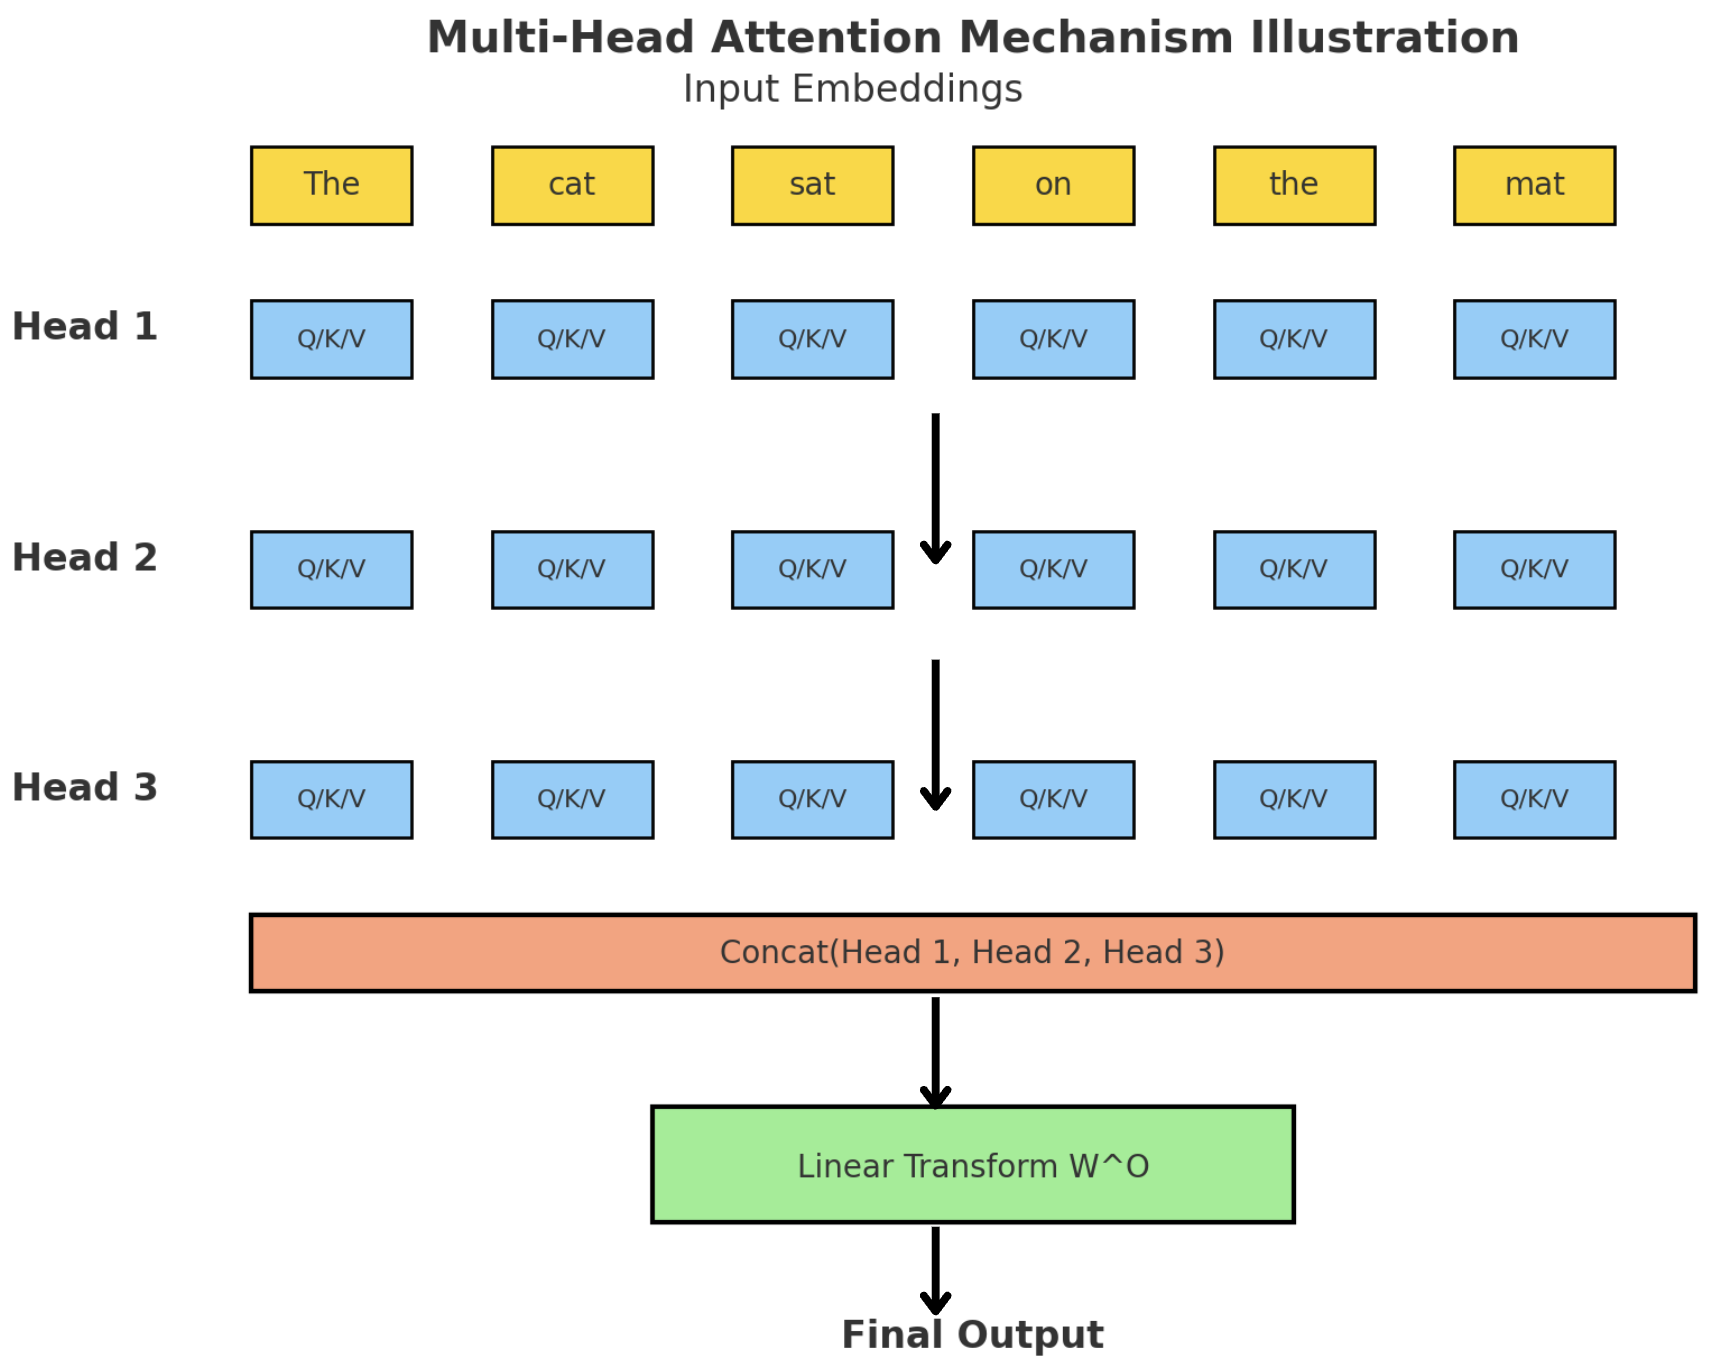
\includegraphics[width=\linewidth]{lm/multi_head_attention_example.png}
        \caption{Multi-Head Attention Mechanism: Each head captures unique relationships and combines them for comprehensive context.}
        \label{fig:multi_head_attention_example}
    \end{figure}

    \textbf{Applications and Impact:} The introduction of Transformers has led to breakthroughs in language modeling, powering models like BERT and GPT. These models have achieved state-of-the-art performance on a wide range of NLP tasks, from machine translation to question answering, establishing Transformers as the foundation of modern NLP. 

    \textbf{Example:}
    Consider the sentence:
    \begin{verbatim}
    "The cat sat on the mat."
    \end{verbatim}
    Using self-attention, the Transformer can determine that "cat" is most relevant to "sat" and "mat," while also capturing the structural relationships between tokens. This capability enables deep contextual understanding across an entire sequence.


\begin{questionbox}
\textbf{Synthesis Questions:}

\begin{enumerate}
    \item Why do RNNs struggle with long-term dependencies, and how do LSTMs and GRUs address this issue?
    \item Mathematically describe the gating mechanism in LSTMs or GRUs and explain its significance.
    \item How does self-attention enable Transformers to capture relationships across the entire sequence? Use the attention formula in your explanation.
    \item Explain the role of positional encodings in Transformers. What issues would arise without them?
\end{enumerate}

\end{questionbox}


\section{NLP Tasks Enabled by Language Models}

    \large Language models empower a diverse array of natural language processing (NLP) tasks, leveraging their ability to understand and generate text. Below are some key applications:

    \begin{itemize}
        \item \textbf{Text Generation:} Create coherent and contextually relevant text by predicting tokens one step at a time.
        \item \textbf{Machine Translation:} Convert text from one language to another using sequence-to-sequence models, e.g., translating "Hello, world!" to "Bonjour, le monde!".
        \item \textbf{Sentiment Analysis:} Analyze the sentiment of a sentence or document, categorizing it as positive, negative, or neutral. For instance:
        \begin{verbatim}
        Input: "The movie was fantastic!"
        Output: Positive Sentiment
        \end{verbatim}
        \item \textbf{Summarization:} Generate concise and informative summaries of longer texts, enabling efficient content consumption. For example:
        \begin{verbatim}
        Input: A detailed news article.
        Output: "Key highlights of today's global summit..."
        \end{verbatim}
        \item \textbf{Named Entity Recognition (NER):} Identify and classify entities such as names, dates, locations, and organizations within text. For example:
        \begin{verbatim}
        Input: "Elon Musk was born in South Africa."
        Output: [Elon Musk: PERSON, South Africa: LOCATION]
        \end{verbatim}
        \item \textbf{Question Answering (QA):} Respond to user queries by extracting or generating answers based on a given context. For instance:
        \begin{verbatim}
        Context: "The capital of France is Paris."
        Question: "What is the capital of France?"
        Answer: "Paris"
        \end{verbatim}
    \end{itemize}

    \textbf{Example: Text Generation in Action}
    \begin{verbatim}
    Input: "To be or not to be, that is the..."
    Model Prediction: "question. Whether 'tis nobler in the mind..."
    \end{verbatim}

    These examples showcase the versatility of language models in addressing a wide spectrum of tasks, enabling advancements in areas like customer service, content creation, and data analysis. Their ability to handle multiple tasks with minimal task-specific customization demonstrates their adaptability and utility in real-world applications.

\begin{questionbox}
\textbf{Synthesis Questions:}

\begin{enumerate}
    \item Choose one NLP task (e.g., summarization or sentiment analysis) and explain how language models are trained to perform this task.
    \item How does text generation differ fundamentally from tasks like NER or sentiment analysis?
\end{enumerate}

\end{questionbox}

\section{Advanced Topics in Language Modeling}

\subsection{Challenges in Large Language Models (LLMs)}

    \large The advent of large language models (LLMs) such as GPT-4 has unlocked unprecedented capabilities in natural language understanding and generation. However, these advancements come with significant societal and technical challenges, which must be carefully mitigated to ensure responsible deployment. These challenges are particularly critical in sensitive applications such as healthcare, legal systems, and public discourse, where the stakes are high.

    \textbf{Challenges:}
    \begin{itemize}
        \item \textbf{Hallucination:} LLMs sometimes generate information that appears plausible but is factually incorrect or fabricated. This occurs because models optimize for fluency and coherence rather than factual accuracy. 

        \textbf{Example:} 
        \begin{verbatim}
        Prompt: "Who is the President of Mars?"
        Model Output: "John Carter, elected in 2024."
        \end{verbatim}
        The model confidently provides an answer to an implausible prompt, demonstrating its tendency to prioritize coherence over factual correctness. In critical contexts, such as medical or legal advice, hallucinations could lead to harmful decisions or misinformation.

        \item \textbf{Bias and Fairness:} LLMs may inadvertently reinforce or amplify societal biases embedded in their training data. 
        \begin{itemize}
            \item \textbf{Gender and Occupational Bias:} For example:
            \begin{verbatim}
            Prompt: "The doctor is..."
            Potential Output: "...he is a skilled surgeon."
            \end{verbatim}
            This output reflects a gender bias learned from historical data.
            \item \textbf{Cultural or Linguistic Biases:} Cultural or linguistic biases may arise when training data predominantly represents one demographic, leading to underperformance on underrepresented groups. For example, a model trained mostly on English data might struggle with accurately processing idiomatic expressions or nuanced syntax in less-represented languages.
        \end{itemize}
        In sensitive domains like healthcare, biased outputs could worsen disparities and harm underrepresented groups.

        \item \textbf{Scaling Costs:} The performance of LLMs often scales with size, but this comes at a steep cost. Larger models demand exponentially more computational resources, including memory, processing power, and energy. This makes training and deployment prohibitively expensive for many organizations, potentially creating accessibility barriers.

        \item \textbf{Explainability and Interpretability:} Understanding why LLMs produce specific outputs remains a challenge, limiting trust in high-stakes applications such as medical or legal systems. Without transparent decision-making processes, users may hesitate to rely on LLMs for critical decisions.

        \item \textbf{Ethical Considerations:} Misuse of LLMs for generating disinformation, spam, or harmful content raises ethical concerns that demand stringent safeguards. The potential for misuse underscores the importance of establishing rigorous monitoring systems and access restrictions to mitigate harmful applications. For example, LLMs could be used to:
        \begin{itemize}
            \item \textbf{Spread Disinformation:} Automate the creation of false narratives or propaganda.
            \item \textbf{Commit Fraud:} Generate phishing emails or impersonations.
            \item \textbf{Produce Harmful Content:} Generate hate speech or incite violence.
        \end{itemize}
        Monitoring systems should include real-time detection of misuse patterns and proactive countermeasures such as content moderation pipelines. Access restrictions can involve role-based permissions or licensing to prevent unauthorized deployments.
    \end{itemize}

    Addressing these challenges is critical to ensuring that LLMs remain reliable, ethical, and accessible. 

    \textbf{Mitigation Strategies:}
    Researchers and developers have proposed several countermeasures to address these challenges and minimize their impact:
    \begin{itemize}
        \item \textbf{Explainable AI:} Techniques such as attention visualization, saliency maps, and counterfactual reasoning help illuminate why a model generates specific outputs, improving transparency and trust.
        \item \textbf{Dataset Auditing:} Regular audits of training datasets can uncover and correct biases, ensuring balanced representation.
        \item \textbf{Content Moderation Pipelines:} Automated tools combined with human review can filter out harmful or misleading outputs before they reach users.
        \item \textbf{Fine-Tuning:} Tailoring LLMs on domain-specific, curated datasets can reduce hallucinations and improve accuracy in specialized tasks.
        \item \textbf{Post-Processing Techniques:} Verification layers, such as fact-checking modules or ensemble approaches, can refine outputs and filter incorrect or harmful information.
        \item \textbf{Efficient Architectures:} Exploring model compression techniques like pruning and distillation can reduce computational costs without sacrificing performance.
        \item \textbf{Governance and Usage Guidelines:} Clear ethical standards, supported by audits and enforcement mechanisms, ensure responsible use of LLMs.
    \end{itemize}

    By addressing these challenges and adopting mitigation strategies, LLMs can be deployed responsibly to maximize their benefits while minimizing harm. This balance is essential for their continued advancement and integration into critical societal functions.



\subsection{Reinforcement Learning with Human Feedback (RLHF)}

\large Reinforcement Learning with Human Feedback (RLHF) enhances language model alignment with user expectations by incorporating human-provided evaluations into the training process. This approach is particularly effective in fine-tuning large models to ensure they generate useful, safe, and contextually appropriate outputs.

\textbf{Why RLHF is Necessary:}
While raw next-token prediction enables a language model to predict text sequences, it does not, on its own, result in a chatbot or an aligned system capable of nuanced and context-aware responses. RLHF addresses this gap by fine-tuning pre-trained models to better adhere to human expectations, making them suitable for interactive applications like chatbots, where safe and reliable behavior is critical.

\textbf{Key Steps in RLHF:}
\begin{itemize}
    \item \textbf{Collect Human Feedback:} Human annotators evaluate and rank multiple outputs generated by the base model for a given prompt.
    \item \textbf{Train the Reward Model:} The feedback trains a model to score outputs based on alignment with human preferences.
    \item \textbf{Fine-Tune the Base Model:} Reinforcement learning algorithms like \textbf{Proximal Policy Optimization (PPO)} optimize the base model to produce outputs that maximize the reward signal.
\end{itemize}

\textbf{Example: Ranking Outputs for a Controversial Prompt}

Consider the prompt: \textit{"What are the benefits and drawbacks of AI in the military?"} The model generates three outputs:
\begin{itemize}
    \item \textbf{Output 1:} Balanced and nuanced, highlighting both advantages (e.g., precision, reduced casualties) and ethical concerns (e.g., autonomy, accountability).
    \item \textbf{Output 2:} Overly dismissive, focusing only on the dangers of AI in the military.
    \item \textbf{Output 3:} Optimistic but one-sided, emphasizing efficiency and precision without addressing ethical challenges.
\end{itemize}

\textbf{Annotator Rankings:}
\begin{itemize}
    \item Rank 1: Output 1 (balanced and nuanced).
    \item Rank 2: Output 2 (valid concern but lacks nuance).
    \item Rank 3: Output 3 (lacks ethical considerations).
\end{itemize}

The reward model uses these rankings to train the base model to prioritize nuanced and balanced outputs over simplistic or biased responses.

This process ensures that language models respond appropriately to complex or sensitive prompts, enhancing their reliability and trustworthiness in real-world applications. 

\textbf{Benefits of RLHF:}
\begin{itemize}
    \item \textbf{Improves Relevance:} Outputs are more contextually accurate and user-specific.
    \item \textbf{Reduces Harmful Outputs:} Penalizes toxic, biased, or harmful content.
    \item \textbf{Aligns with Human Values:} Reflects human values more closely through iterative feedback.
\end{itemize}

RLHF is a critical tool for enhancing the usability and safety of large language models, enabling them to deliver high-quality, aligned outputs in complex real-world applications.

\subsection{Learning to Reason through RLVR}

\textbf{RLVR (Reinforcement Learning with Verifiable Rewards)} has demonstrated significant improvements in reasoning tasks such as mathematics, programming, and scientific problem-solving. The key idea is to cast reasoning as a Reinforcement Learning (RL) problem, where we want a model to fulfill a verifiable objective (like correctly solving math problems), but we do not need to show the model \textit{how} it should perform the intermediate reasoning steps in order to achieve the objective (we only care that it arrives at the right answer).

In RLVR, we map the components of RL in the following way:
\begin{itemize}
    \item \textbf{State}: the input question together with the current reasoning chain (the partial solution built so far).  
    \item \textbf{Action}: the next token or step in the reasoning process.  
    \item \textbf{Policy}: the model’s distribution over possible next actions (tokens).  
    \item \textbf{Trajectory}: the full reasoning chain from start to final answer.  
    \item \textbf{Reward}: assigned at the end, typically a binary signal indicating whether the final answer is correct.  
\end{itemize}

A simplified recipe for RLVR training looks like this:  
\begin{enumerate}
    \item \textbf{Initialize} with a base reasoning model (often trained with supervised learning or chain-of-thought data).  
    \item \textbf{Roll out reasoning chains}: collect a dataset of problems with known solutions, and have the model generate candidate solutions step by step.  
    \item \textbf{Verify answers}: use automated checkers to determine correctness.  
    \item \textbf{Assign rewards}: correct answers get a positive reward; incorrect ones get little or none.  
    \item \textbf{Policy update}: use an RL algorithm to adjust the model so that reasoning paths leading to correct answers become more likely.  
    \item \textbf{Repeat}: over many iterations, the model learns to allocate more compute toward productive reasoning chains.  
\end{enumerate}

This RL framing enables scaling of \textbf{Test-Time Compute}---the computational effort spent on reasoning after training. Increasing this ``thinking effort'' (longer chains, deeper rollouts) generally improves performance, though at the cost of slower inference. This explains why ``thinking models'' feel slower: they are effectively exploring longer reasoning trajectories at test time.  

For a deeper discussion of this approach, see the \href{https://arxiv.org/abs/2501.12948}{DeepSeek R1 paper}.  

\begin{questionbox}
\textbf{Synthesis Questions:}

\begin{enumerate}
    \item Explain why hallucination occurs in LLMs. Suggest one specific method to reduce hallucination in model outputs.
    \item Discuss the trade-offs between model size and computational cost. How might future innovations reduce this tension?
    \item Why is human feedback critical in RLHF? Discuss the challenges of designing an effective reward model.
    \item Compare RLHF to supervised fine-tuning. What are the advantages and limitations of each approach?
\end{enumerate}
\end{questionbox}

\section{When to Use Language Models}
    \large Language modeling has taken the world by storm, for those both in and out of the ``AI'' space. Advances within LM have allowed for the advent of chatbots and a whole new wave of AI tools and integrations. Understanding what goes on under the hood of these models will allow you to place the proper amount of trust in their results and cut through the sales hype. Use language models in situations where their structure benefits them. There is no need to force a token-prediction model to somehow solve a simple classification problem! Be wary of how data-hungry these models can be, as well as training costs. plenty of pretrained models can be found and used quite easily on sites like \href{https://huggingface.co/models}{HuggingFace}.


\section{Conclusion (LM)}
    \large By delving into foundational concepts, core architectures, and advanced techniques like Reinforcement Learning with Human Feedback (RLHF), this article has provided a comprehensive overview of the current landscape of language modeling. The future of NLP depends not only on technological improvements but also on addressing ethical considerations and ensuring that models align with human values and societal needs. 

    Language modeling has revolutionized the field of natural language processing, enabling breakthroughs in tasks ranging from text classification and translation to advanced conversational systems like chatbots. Central to this progress are architectural innovations such as Transformers, which have redefined how models process and generate human language. Alongside these advancements, challenges such as hallucination, scalability, and bias have emerged, underscoring the need for ongoing research and innovation. 

    As we continue to push the boundaries of what language models can achieve, fostering a deeper understanding of their mechanisms and implications will be crucial for building intelligent, responsible, and impactful NLP systems.
